\documentclass{article}

\usepackage[utf8]{inputenc}
\usepackage[T1]{fontenc}

% If the output is a PDF (avoids some display problems, in particular in arXiv).
\pdfoutput = 1


% This is the file kl-minimal.tex.
% It can be used as a starting point for creating a document using the _knowledge_ package.
%
% The documentation of the _knowledge_ package can be found:
% - in your tex distribution, using the command
%        texdoc knowledge
% - or at the address
%.       https://ctan.org/pkg/knowledge
%
%
% Loading other packages before knowledge activates features.
% The most common use of knowledge makes use of hyperref and xcolor:
\usepackage[breaklinks]{hyperref} 
\usepackage{cleveref} 
\usepackage{xcolor} 
%
% The package 'knowledge' has now to be loaded.
% The options 
%      'paper', 'electronic' or 'composition' (default)
% can be used. These activates different rendering styles:
% - 'paper' produce a paper to be printed:
%   text in black and white
% - 'electronic' highlights links using colors:
%   for being read on an electronic device
% - 'composition' (or default) highlights missing knowledges as
%   well as gives other pieces of information. It should always
%   be used but when the paper is ready.
%
\usepackage{knowledge} % default
%\usepackage[electronic]{knowledge} % final version to be read electronically
%\usepackage[paper]{knowledge} % final version in black and white for printing

% The 'notion' configuration is commonly used for scientific papers.
% The 'quotation' configuration is commonly used and triggers the "..." notation.
\knowledgeconfigure{notion, quotation}

% It is convenient to provide a list of knowledges in an external file.
\knowledge{url={https://ctan.org/pkg/knowledge}, typewriter}
 | knowledge@package

\knowledge{url={http://mirrors.ctan.org/macros/latex/contrib/knowledge/knowledge.pdf}}
 | documentation

\knowledge{url={https://ctan.org/pkg/hyperref?lang=en}, typewriter}
 | hyperref

\knowledge{text=\LaTeX}
 | latex

\knowledge{notion}
 | Knowledges@concept
 | knowledge@concept
 | knowledges@concept

\knowledge{notion}
 | Directives
 | directives
 | directive

\knowledge{notion, typewriter}
 | notion
 | notions

\knowledge{url={https://en.wikipedia.org/wiki/Tomato}, color=purple, boldface}
 | tomato
 | tomatoes
 | Tomato
 | Tomatoes

\knowledge{notion}
 | introduce
 | introduced
 | introduction

\knowledge{notion}
 | anchor points

\knowledge{notion}
 | composition mode

\knowledge{notion}
 | paper mode

\knowledge{notion}
 | electronic mode

\knowledge{notion}
 | scopes

% It is convenient to provide a list of macros in an external file.
\knowledgenewrobustcmd\automata{\cmdkl{\mathcal{A}}}

\knowledgenewrobustcmd\interval[2]{
    \cmdkl{[} #1, #2 \cmdkl{]}
}


\usepackage{graphicx}


\title{A tutorial for the "knowledge@@package" package}
\author{Enthusiastic users of the "knowledge@@package" package}
\date{\today}


\begin{document}

\maketitle

\begin{abstract}
    This is a tutorial on how to to use the 
    "knowledge@@package" package, together with "knowledge-clustering".
    It shows the basic features of the package, namely how 
    to introduce internal and external hyperlinks on text and math commands,
    as well as more advanced features.
    It also contains a guide on how to install and use "knowledge-clustering", 
    a ``nifty software tool'' that aims to ease the use of "knowledge@@package".
\end{abstract}

\tableofcontents

\section{Introduction}

The package \AP""knowledge@@package"" is a package for "latex" that helps associating 
information to terms. It can be used for:
\begin{itemize}
    \item managing external urls, for instance separating the file containing   
        the addresses from their use,
    \item managing internal references's such as linking every use of a concept 
        to the place of its introduction
        (in particular avoiding the use of labels),
    \item managing the index in a centralized way,
    \item replacing some macros.
\end{itemize}

Primarily, the goal of the "knowledge@@package" is for the production of scientific documents (the longer, the more interesting, such as a thesis or a book) in order to improve their readability on electronic devices. Ultimately, the goal is to produce documents that are more semantic-aware.

Throughout this document, we will refer to the "knowledge@@package" 
"documentation". It can be accessed localy by typing \verb|texdoc knowledge| in 
a prompt, or "online@documentation".

To use "knowledge@@package" in your "latex" document, write in the preamble:
\begin{verbatim}
    \usepackage[breaklinks]{hyperref} 
    \usepackage{xcolor} 

    \usepackage{knowledge}

    \knowledgeconfigure{notion, quotation}
\end{verbatim}

By default, "knowledge@@package" is loaded in \AP""composition mode"", which renders 
links and warnings. The document can be switched to the \AP""paper mode""
which is made for printing (links still exist but are displayed in black)
or \AP""electronic mode"" (links are colored, warnings and "anchor points"
are hidden), by writing \verb|\usepackage[paper]{knowledge}|
or \verb|\usepackage[electronic]{knowledge}|, respectively.

\section{Basic features}

Try compiling this document (two compilation phases to have proper links) using pdflatex, and see how some notions are hyperlinked to their introduction point (some viewers make it more obvious than others by displaying a preview of the target of a link inside a document).

\subsection{Aesthetical changes and external links}

\AP""Knowledges@@concept"" are the key concept in the "knowledge@@package" 
package. Essentially, a "knowledge@@concept" corresponds to a concept used in 
the document. To invoke a "knowledge@@concept" named ``tomato'', one simply has 
to write \verb|\kl{tomato}| (or simply
\knowledgeconfigure{quotation=false}%
\verb|"tomato"|%
\knowledgeconfigure{quotation=true}%
if the 'quotation' 
configuration is enabled) in their document. At compilation, this will 
print the text ``tomato'' and apply (aesthetical or semantical) changes that
are associated with the "knowledge@@concept" ``tomato''.

To specify what modifications should be performed on a "knowledge@@concept", 
you must define it, either in the beginning of your document or in an external file (in \texttt{notions.tex} in this example) included in your preamble.
The basic syntax to do so is
\begin{verbatim}
    \knowledge{}
     | tomato
\end{verbatim}
\AP""Directives"" can be written between the pair of brackets. A complete list of "directives" can be found in §5.3 of the "knowledge@@package" "documentation". Most basic example include:
\begin{itemize}
    \item \verb|url=<LINK>| to add an external hyperlink;
    \item \verb|color=<COLOR>| to change the color of the "knowledge@@concept";
    \item \verb|italic| and \verb|up| to force/unforce italic;
    \item \verb|boldface| and \verb|md| to force/unforce boldface;
    \item \verb|smallcaps| to force small capitals;
    \item \verb|underline| to underline;
    \item \verb|lowercase| and \verb|uppercase| to render the text in lowercase or uppercase;
    \item \verb|typewriter| to render the text in typewriter.
    \item \verb|text=<TEXT>| to change the text that is displayed.
\end{itemize}

You will often want to define synonyms, i.e. to have multiple names associated to a single "knowledge@@concept": for instance you might want ``tomatoes'', ``Tomato'' and  ``Tomatoes'' to all refer to the same "knowledge@@concept" as ``tomato''. This can be achieved by defining each synonym on a new line, precedeed by a pipe. For example
\begin{verbatim}
    \knowledge{url={https://en.wikipedia.org/wiki/Tomato},
        color=purple, boldface}
     | tomato
     | tomatoes
     | Tomato
     | Tomatoes
\end{verbatim}
will produce the following result when one writes \verb|\kl{Tomatoes}| or
\knowledgeconfigure{quotation=false}%
\verb|"Tomatoes"|%
\knowledgeconfigure{quotation=true}:%
\begin{quote}
    "Tomatoes"
\end{quote}
namely it will write the text ``Tomatoes'' in bold, purple, and insert a link to the Wikipedia page named ``Tomato''.


\subsection{Internal hyperlinks: the "notion" directive}

The ""notion"" "directive" allows you to easily introduce internal hyperlinks.
Say that you have defined a "knowledge@@concept"
\begin{verbatim}
    \knowledge{notion, <OTHER_DIRECTIVES>}
     | name
     | synonym
\end{verbatim}
By writting \verb|\intro{name}| (or
\verb|\intro{synonym}|, or 
\knowledgeconfigure{quotation=false}%
\verb|""name""|, or \verb|""synonym""|%
\knowledgeconfigure{quotation=true}%,
) you will \AP""introduce"" your knowledge. Then, whenever you will write
\verb|\kl{name}| (or
\verb|\kl{synonym}|, or 
\knowledgeconfigure{quotation=false}%
\verb|"name"|, or \verb|"synonym"|)%
\knowledgeconfigure{quotation=true}
"knowledge@@package" will add an internal hyperlink to the place where
your "notion" was "introduced". The default behaviour\footnote{Inherited from
"hyperref".} is to add a link to the beginning of the section in which the "notion" was introduced. Since this is very often unsatisfying, the command
\verb|\AP| allows you to define custom \AP""anchor points"", depicted as 
small red corners in the left margin of your document when you are in "composition mode".
Internal hyperlinks 
will refer to the last anchor point preceding the "introduction" of your 
"notion".

By default, "notions" appear in blue, and "introduction" of "notions"
appear in dark blue and italics.
Note that a single "notion" should only be introduced once (even if you have synonyms). Should you want to reintroduce an already introduced "notion", 
you can use the \verb|\reinto{...}| command.

\subsection{Scopes and extended syntax}

Sometimes the same piece of text can refer to different concepts: for example, in this document, ``knowledge'' refers both to the "knowledge@@package" package
and to the concept of "knowledges@@concept". In this case, \AP""scopes"" allow 
you to distinguish these concepts, by defining the two "knowledges@@concept"
\begin{verbatim}
    \knowledge{url={https://ctan.org/pkg/knowledge}, typewriter}
     | knowledge@package

    \knowledge{notion}
     | knowledge@concept
\end{verbatim}
To invoke one or the other, you can write
\knowledgeconfigure{quotation=false}%
\begin{verbatim}
    "knowledge@@scope"
        or
    \kl(scope){knowledge}
\end{verbatim}
\knowledgeconfigure{quotation}%
where \verb|scope| is either \verb|package| or
\verb|concept|.
More informations on "scopes" can be found in §3.5 of the "documentation".

Finally, if you want to display some ``text'' that behaves
like some "knowledge@@concept" named ``name'', you can write
\knowledgeconfigure{quotation=false}%
\begin{verbatim}
    "text@name"
        or
    \kl[name]{text}
\end{verbatim}
\knowledgeconfigure{quotation}%
This is useful when you do not want ``text'' to be a synonym
of ``name'' throughout the paper but only locally.
For instance,
\knowledgeconfigure{quotation=false}%
\begin{verbatim}
    (...) "These vegetables@tomato" are (...)
\end{verbatim}
\knowledgeconfigure{quotation}%
produces 
\begin{quote}
    (...) "These vegetables@tomato" are (...)
\end{quote}
namely the style of the "knowledge@@concept" ``tomato'' is applied to the
string ``These vegetables''.


\subsection{Mathematical commands}


The previous sections can mostly be applied to mathematical commands:
for instance 
\begin{verbatim}
    $\kl[tomato]{\Pi^P_2}$
\end{verbatim}
will produce $\kl[tomato]{\Pi^P_2}$. However, as a rule of thumb,
this should be avoided as there is a more elegant syntax for 
knowledgyfied mathematical commands. It is recommanded to
use semantic macros instead of syntactic ones: for example,
instead of defining a macro \verb|\Ac| that displays $\mathcal{A}$, 
define \verb|\automata| or \verb|\algebra|.

The basic syntax to define a new mathematical command is:
\begin{verbatim}
    \knowledgenewrobustcmd<COMMAND_NAME>{\cmdkl{
        <YOUR_MACRO>
    }}
\end{verbatim}
for example
\begin{verbatim}
    \knowledgenewrobustcmd\automata{\cmdkl{
        \mathcal{A}
    }}
\end{verbatim}
defines a macro named \verb|\automata| that prints an `$\mathcal{A}$' and 
defines a "notion" named \verb|\automata|.
Using the command \verb|\automata| (e.g: $\automata$) will result in
"knowledge@@package" automatically inserting a link to the last "anchor point"
preceding the introduction of the "notion" \verb|\automata|.
This notion can be introduced by writting
\begin{verbatim}
    \intro*\automata
\end{verbatim}
which produces the following result: $\AP\intro*\automata$.

The \verb|\cmdkl| command allows you to control which part of the macro will be
knowledgyfied/cliquable. For instance, if you define the macro
\AP\phantomintro{\interval}
\begin{verbatim}
    \knowledgenewrobustcmd\interval[2]{
        \cmdkl{[} #1, #2 \cmdkl{]}
    }
\end{verbatim}
then \verb|$\interval{a}{b}$| will produce $\interval{a}{b}$: only the two
brackets will be cliquable.


\section{Knowledge-Clustering}

\subsection{Goal}

"Knowledge-clustering" is a command-line tool that aims to automate part of
the process of writting a document with "knowledge@@package".
As of today, "knowledge\-clustering" has to main features:
\begin{itemize}
    \item the "clustering" feature, which automates the definitions
    of synonyms. For example,  if at some point you already defined the 
    "knowledge@@concept" \verb|tomato| and write in your document
    \knowledgeconfigure{quotation=false}%
    \verb|"Tomatoes"|
    \knowledgeconfigure{quotation}%
    then, at compilation, "latex" will rightfully produce a warning,
    saying that the knowledge \verb|Tomatoes| is undefined.
    At this point, you should run "knowledge-clustering", which will propose to 
    you to define \verb|Tomatoes| as a synonym of \verb|tomato|.
    \item the "add quotes" feature, that can be used at the very end of your 
    writting process, to check if every piece of text that is defined as
    a "knowledge@@concept" is surronded by quotes. For example, this feature 
    \knowledgeconfigure{quotation=false}%
    would suggest to replace the string \verb|Let $x$ be a tomato such that (…)|
    in you \verb|.tex| file by \verb|Let $x$ be a "tomato" such that (…)|.
    \knowledgeconfigure{quotation}%
\end{itemize}

\subsection{Installation}

To install "knowledge-clustering", you need to have a machine with
\verb|python3| and \verb|pip3|. To install, or upgrade, "knowledge-clustering",
you can simply run
\begin{verbatim}
    pip3 install --upgrade knowledge-clustering
\end{verbatim}
in your shell.
Then, you should run
\begin{verbatim}
    knowledge init
\end{verbatim}
to download some data, used by the "clustering" algorithm\footnote{This 
downloads some data used by "NLTK", a natural language package used by 
"knowledge@@package".}.

\paragraph{Autocomplete}
If the autocomplete of the command \verb|knowledge| does not work,
you can follow the following procedure:
if you are using \verb|zsh| (resp. \verb|bash|), then add
\knowledgeconfigure{quotation=false}%
\begin{verbatim}
    eval "`pip completion --zsh`"
\end{verbatim}
or 
\begin{verbatim}
    eval "`pip completion --bash`"
\end{verbatim}
\knowledgeconfigure{quotation}%
in your \verb|.zshrc| file (resp. \verb|.bashrc|).
For the change to take effect, you either need to launch a new terminal,
or run \verb|source ~/.zshrc| (resp. \verb|source ~/.bashrc|).

\subsection{Clustering knowledges}

\subsubsection{Basic use}

The \AP""clustering"" feature is meant to be used
when you are writing you "latex" document with "knowledge@@package".
Maintaining the list of all the "knowledges@@concept" you're using
can be burdersome, so usually you will write your "latex" code
and use, in this code, some "knowledges@@concept" that are yet to be
defined.

\begin{figure}[htb]
    \centering
    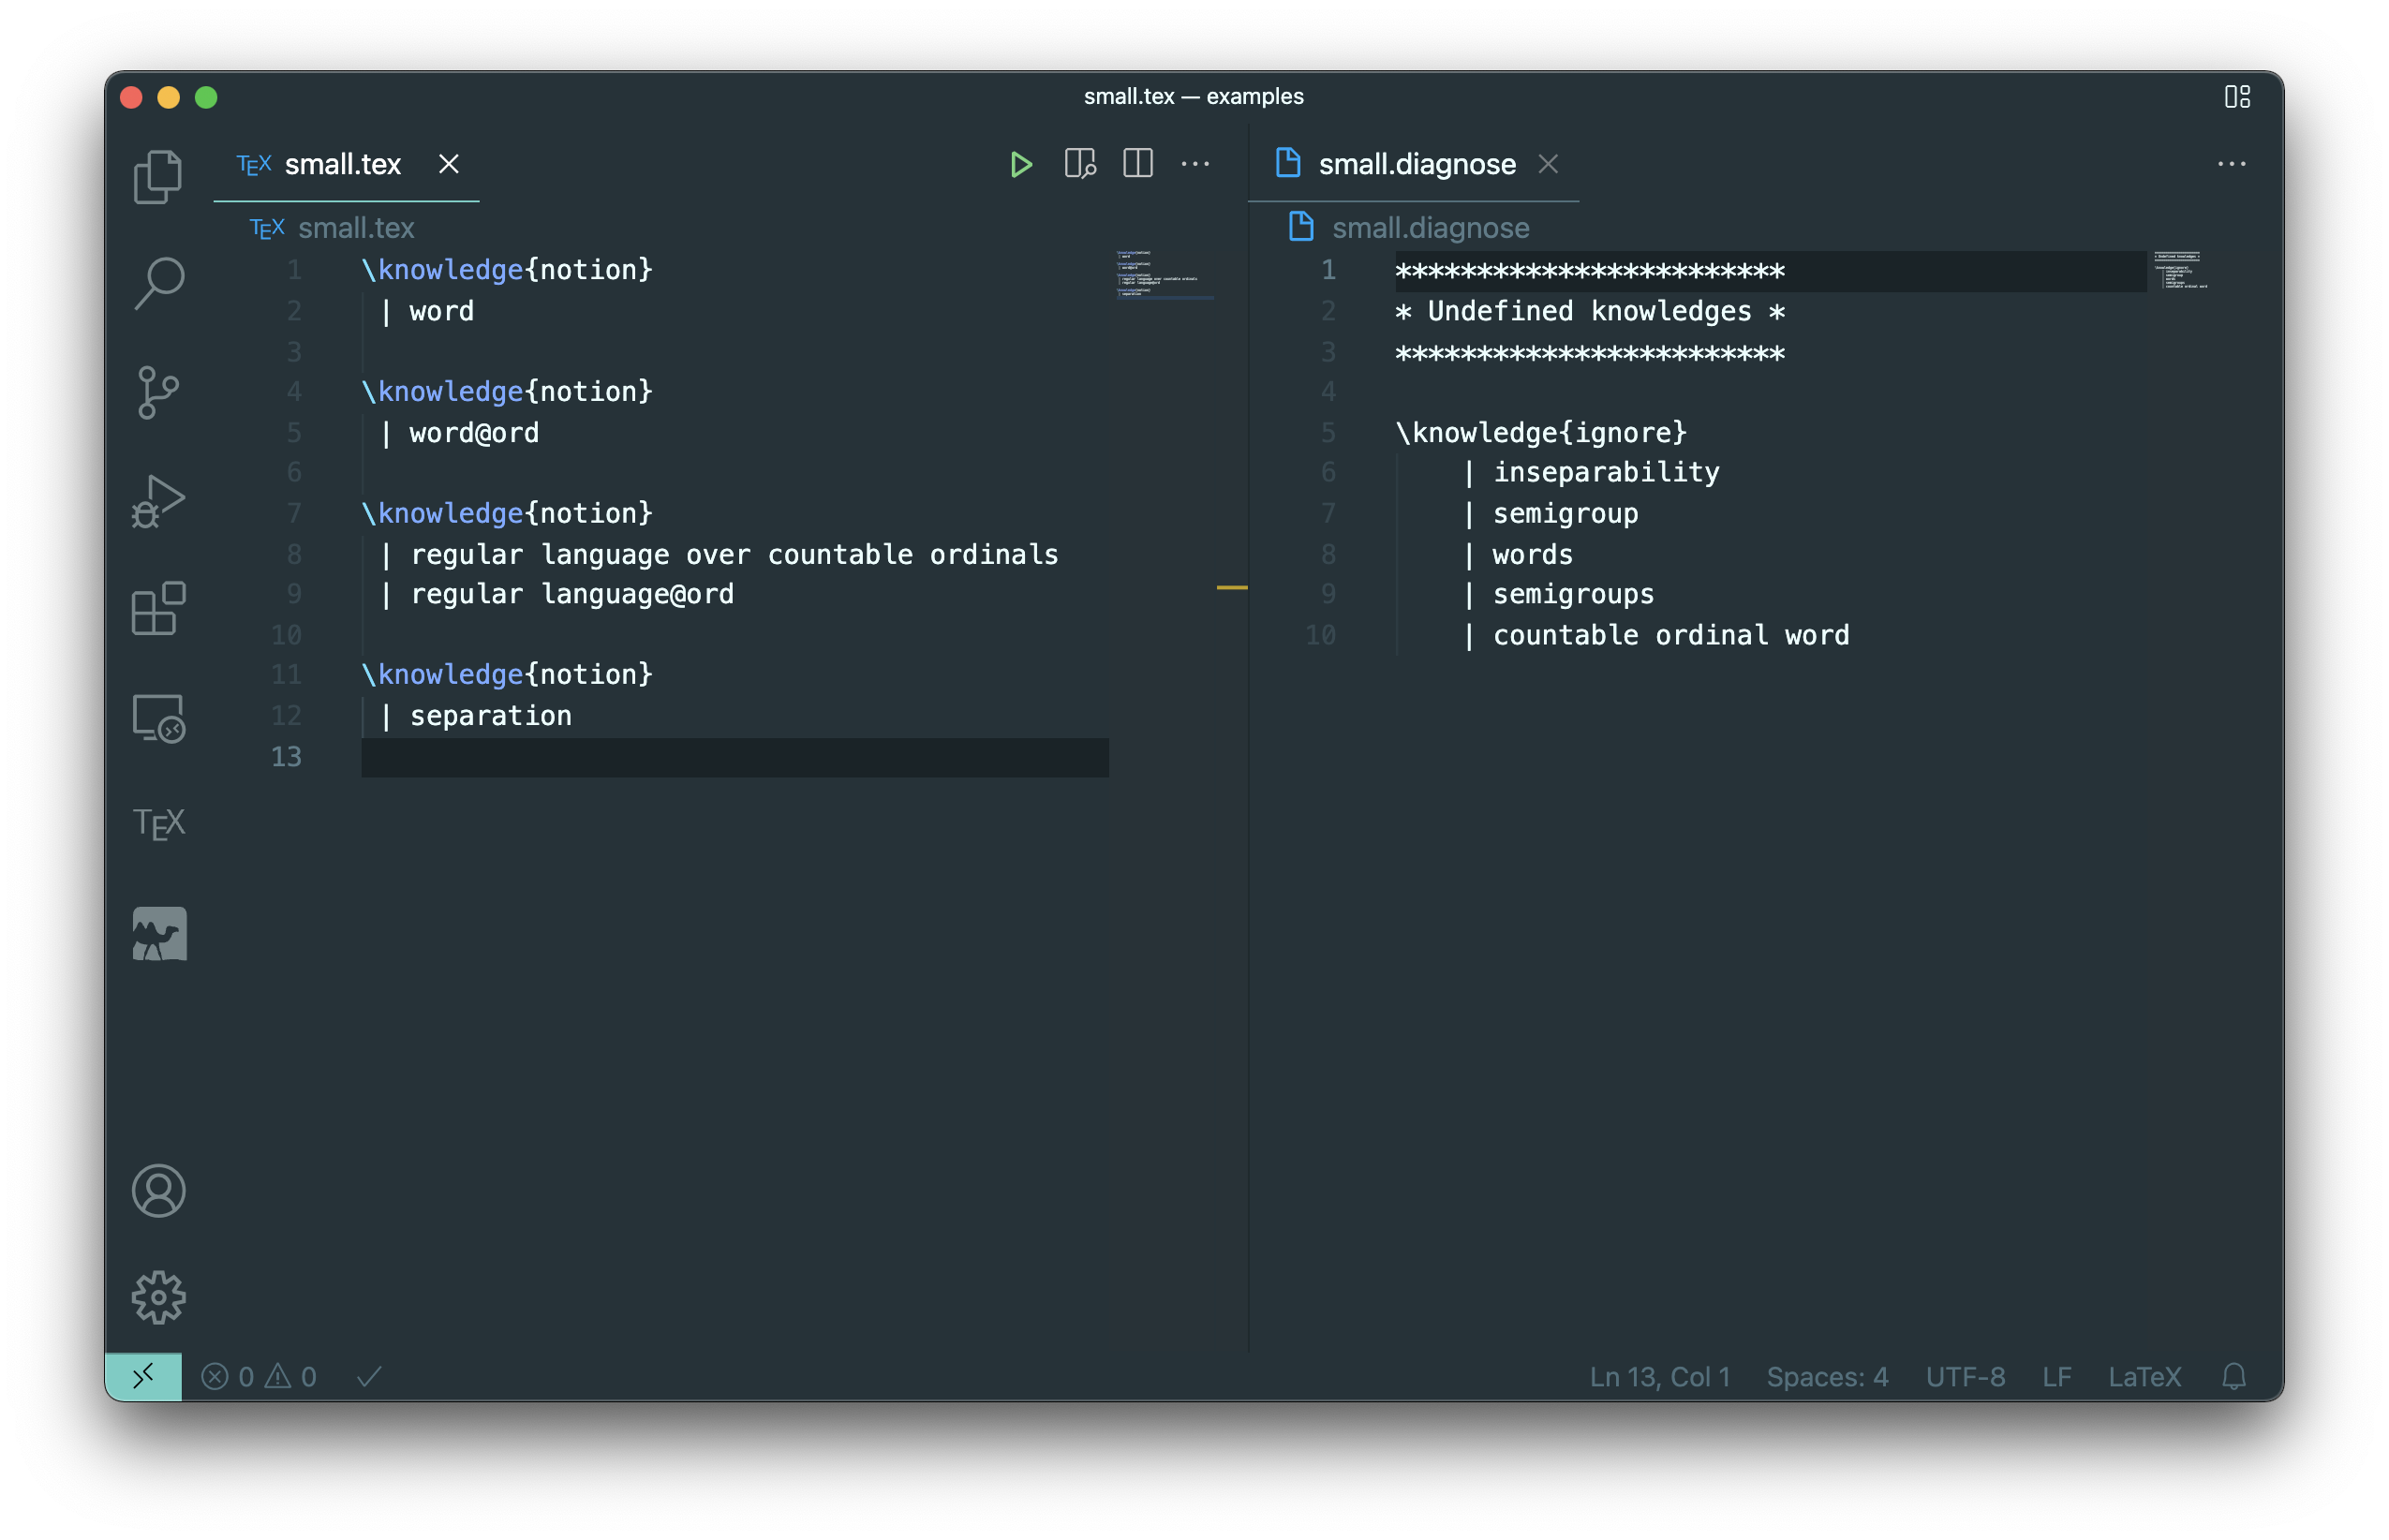
\includegraphics[width=.9\textwidth]{img/small-before.png}
    \caption{%
        \label{fig:clustering-before}
        Content of the file containing the defined "knowledges@@concept"
        (left-hand side) and of the \texttt{.diagnose} file produced by
        "latex" at compilation (right-hand side), before running 
        "knowledge-clustering".
    }
\end{figure}

For example, \Cref{fig:clustering-before} illustrates the following situation:
in the file containing all your defined "knowledges@@concept", you have
four "knowledges@@concept", one of which is ``\verb|word|''.
In your main \verb|.tex| file---which is not reproduced here---, you used some 
undefined "knowledges@@concept", such as ``\verb|words|'' and
``\verb|semigroup|''.
At compilation, "latex" will produce a warning, saying that you have undefined
"knowledges@@concept", and write in a \verb|.diagnose| file a list
of these undefined "knowledges@@concept".

At this point, you have two options: you can either define every undefined "knowledge@@concept", by hand, and say that ``\verb|words|'' is a synonym of
``\verb|word|'' while ``\verb|semigroup|'' is a new "knowledge@@concept".
Or, you can use the "clustering" feature of "knowledge-clustering": feed
it both files (the file \verb|small.tex| containing the defined 
"knowledges@@concept" and
the \verb|small.diagnose| file containing the undefined "knowledges@@concept")
by running the command
\begin{verbatim}
    knowledge cluster -n small.tex -d small.diagnose
\end{verbatim}
which will write suggestions in your file \verb|small.tex|,
as depicted in \Cref{fig:clustering-after}. These suggestions
take the form of comments: if you agree with the suggestion, you can just
uncomment the line, and otherwise, you should move it, by hand.

\begin{figure}[htb]
    \centering
    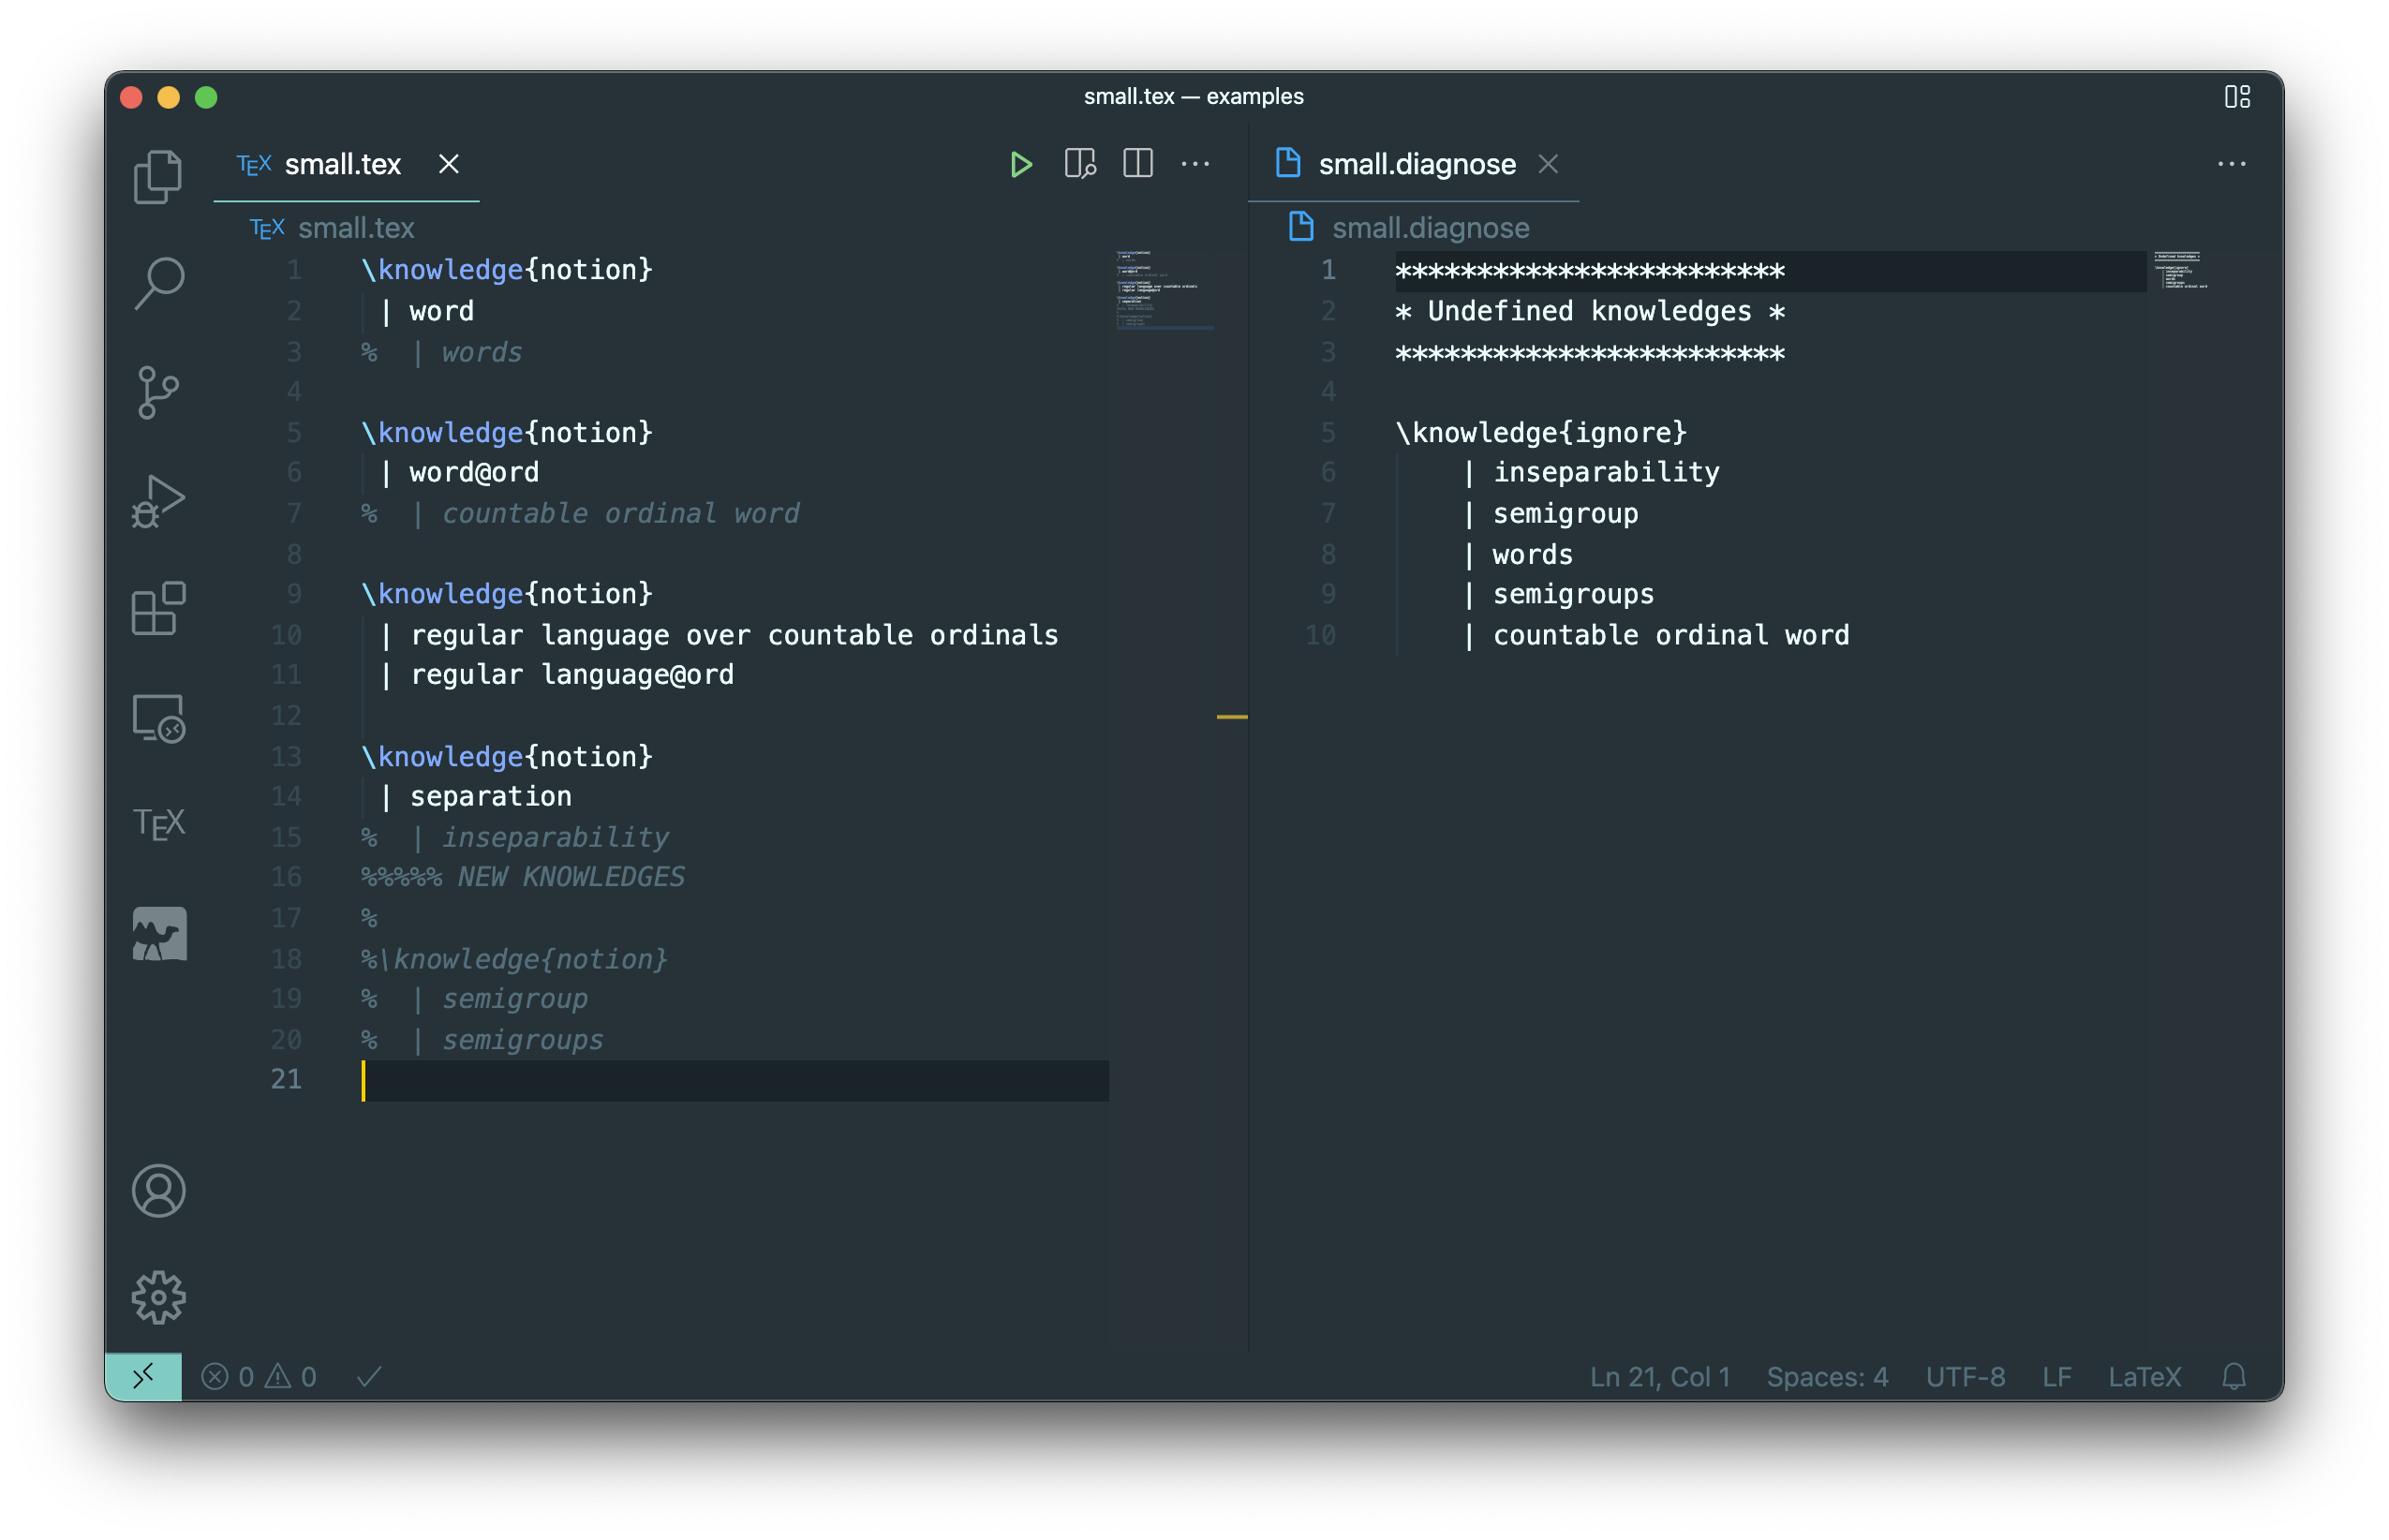
\includegraphics[width=.9\textwidth]{img/small-after.png}
    \caption{%
        \label{fig:clustering-after}
        After running "knowledge-clustering", the \texttt{small.diagnose} file
        is left unchanged, while \texttt{small.tex} now contains suggestions
        of how to define the new "knowledges@@concept".
     }
\end{figure}


\subsubsection{Advanced features}

To display the help, you can run \verb|knowledge cluster --help|.

\paragraph{Language} The "clustering" algorithm relies on natural language 
processing and is language-specific. As of today, only two languages
are supported: english (which is the default language) and french.
To use "knowledge-clustering" on a document written in french,
simply add \verb|-l fr| or \verb|--lang fr| at the end of your command.


\paragraph{Scopes} In the example of
\Cref{fig:clustering-before,fig:clustering-after}
you can see that "knowledge-cluste\-ring" infered that the
scope ``ord'' meant ``countable ordinals''\footnote{This was infered
by reading the \texttt{small.tex} file, and was used to cluster
the "knowledge@@concept" ``countable ordinal word'' with ``word@ord''.}.
If you want the list of scopes it saw,
and of their infered meaning, you can use the \verb|-S| or \verb|--scope| 
option. 
For instance, running
\begin{verbatim}
    knowledge cluster -n small.tex -d small.diagnose --scope
\end{verbatim}
will print in your prompt
\begin{verbatim}
    Defined scopes:
	    @ord : [['ordinals', 'countable'], ['ord']]
\end{verbatim}


\subsection{Forgotten quotes}


The "add quotes" feature is meant to be used when your document is (nearly)
finished and you want to check that you have not forgotten ``quotes'' symbols
(or a \verb|kl{}| command) before and after defined "knowledges@@concept".

The basic syntax is the following:
\begin{verbatim}
    knowledge addquotes -t <TEX_FILE> -n <NOTION_FILE> 
\end{verbatim}
where:
\begin{itemize}
    \item \texttt{<TEX\_FILE>} is the \verb|.tex| file containing your "latex"
    document :
    \item \texttt{<NOTION\_FILE>} is the file containing the
    "knowledges@@concept" you have defined.
\end{itemize}
Then, your prompt will display something like
\begin{verbatim}
    Found a match for `blabla` at line 41.
    Add quotes? [y/n]
\end{verbatim}
Depending on your answer, the "add quotes" feature will add a quote
\knowledgeconfigure{quotation=false}%
\verb|"| before, and a quote \verb|"| after 
\knowledgeconfigure{quotation}%
the piece of text ``blabla'' found at line 41.

The only available option is \verb|-F| or \verb|--force| to add
quote symbols around every match. It is \textbf{highly discouraged}
to use this feature. 

\subsection{Contributing to "knowledge-clustering"}

If you have bugs to report or suggestions, you can submit a
\href{https://github.com/remimorvan/knowledge-clustering/issues}{new issue},
or a new pull request on github, or get in touch by email with
one of the maintainers.


\section{Advanced features}

This section is dedicated on more advanced features of "knowledge@@package".

\subsection{Weird spacing for math commands}

\subsection{Disabling commands}

\subsection{Changing the default colors}



\end{document}